\documentclass[10pt,a4paper]{article}
\usepackage[T1]{fontenc}
\usepackage[utf8]{inputenc}
\usepackage[english]{babel}
\usepackage{lmodern,microtype}
\usepackage[a4paper,margin=1.8cm,headheight=15pt]{geometry}
\usepackage{enumitem,tabularx,array,longtable,booktabs,xcolor,hyperref,xurl,fancyhdr,titlesec,framed,listings}
\usepackage{tikz}
\usetikzlibrary{arrows.meta,positioning,calc}
\definecolor{ddtadark}{RGB}{28,38,52}
\definecolor{ddtablue}{RGB}{42,88,135}
\definecolor{ddtagray}{RGB}{244,246,248}
\definecolor{ddtaorange}{RGB}{148,91,25}
\definecolor{ddtagreen}{RGB}{48,111,78}
\definecolor{ddtared}{RGB}{140,48,48}
\hypersetup{colorlinks=true,linkcolor=ddtablue,urlcolor=ddtablue,pdftitle={BA0-T1 FR-3.4 application trial R1}}
\pagestyle{fancy}\fancyhf{}\lhead{DDTA - BA0-T1}\rhead{FR-3.4 application trial R1}\cfoot{\thepage}
\titleformat{\section}{\large\bfseries\color{ddtadark}}{\thesection}{.6em}{}
\titleformat{\subsection}{\normalsize\bfseries\color{ddtadark}}{\thesubsection}{.6em}{}
\setlist[itemize]{leftmargin=1.45em,itemsep=.12em,topsep=.2em}
\setlist[enumerate]{leftmargin=1.7em,itemsep=.12em,topsep=.2em}
\setlength{\parindent}{0pt}\setlength{\parskip}{.30em}\setlength{\emergencystretch}{2em}
\lstset{basicstyle=\ttfamily\small,frame=single,breaklines=true,backgroundcolor=\color{ddtagray}}
\newenvironment{trialbox}[1]{\def\FrameCommand{\fcolorbox{ddtaorange}{ddtagray}}\MakeFramed{\advance\hsize-2\width\FrameRestore}\noindent\textbf{#1}\par\smallskip}{\endMakeFramed}
\newenvironment{resultbox}[1]{\def\FrameCommand{\fcolorbox{ddtagreen}{ddtagray}}\MakeFramed{\advance\hsize-2\width\FrameRestore}\noindent\textbf{#1}\par\smallskip}{\endMakeFramed}
\newenvironment{warningbox}[1]{\def\FrameCommand{\fcolorbox{ddtared}{ddtagray}}\MakeFramed{\advance\hsize-2\width\FrameRestore}\noindent\textbf{#1}\par\smallskip}{\endMakeFramed}
\newcolumntype{Y}{>{\raggedright\arraybackslash}X}
\begin{document}
\begin{center}
{\LARGE\bfseries BA0-T1 concrete application trial}\par
{\large FR-3.4 Deliver RecognitionCapture - Revision 1}\par\smallskip
{\small Repository baseline: \texttt{bc0143eb8493ca91d3094eca9f8fbf9c7e6a3e58}}
\end{center}

\begin{trialbox}{Status: COMPLETED TRIAL / PROVISIONAL / BA0 NOT CLOSED}
This trial applies the BA0 working hypothesis to one concrete facial-access fragment before any BAE taxonomy is designed. Trial identifiers are not metaclasses and no BAE type is accepted here.
\end{trialbox}

\section{What is being tested}
The practical question is: which analytical knowledge must be made explicit around \texttt{FR-3.4} so that the same system meaning can be reused across analysis consumers and controlled mutations?

The pinned source is:
\begin{lstlisting}
04-specialized-requirement/03-example-facial-access/
DDTA_FACIAL_ACCESS_CAMERA_S1_STUDY_CORPUS_R2.tex
blob d54fdecc7d4968a88b74ea96343b37f38bb9b6d1
\end{lstlisting}

The source is an experimental DDTA study corpus. In this trial, ``grounded'' means directly supported by this pinned corpus, not production-system truth.

\section{Source basis}
\begin{itemize}
\item \textbf{D-3.3}: \texttt{CameraSubsystem} acquires evidence; a distinct local \texttt{RecognitionProcessor} performs recognition. The decision explicitly creates a responsibility separation and requires evidence to cross it.
\item \textbf{FR-3.4}: \texttt{CameraSubsystem} delivers each remotely evaluated \texttt{RecognitionCapture} to \texttt{RecognitionProcessor}, correlates it with the correct \texttt{RecognitionRequest}, and must not report incomplete delivery as success.
\item \textbf{D-3.4}: the project consumes local connectivity and does not own/manage the underlying transport infrastructure.
\item \textbf{D-3.5}: current connectivity realization is wired Ethernet.
\item \textbf{SR-3.4-C/I/P}: confidentiality, integrity and authorized-origin conditions apply to the FR-3.4 delivery/acceptance context.
\end{itemize}

The corpus also provides two mutations used here: M1 Ethernet to Wi-Fi, and M3 remote recognition to local recognition.

\section{Trial notation}
\begin{lstlisting}
T-Rxx = provisional referent an analysis may need to distinguish
T-Sxx = provisional analytical statement about referents
T-Xxx = proposed analytical addition used as a falsification probe

G = grounded in selected source statement
D = derived analytical normalization, no new project commitment
A = analytical addition not asserted/entailed by the source
C = conflicting source support
\end{lstlisting}

Identity pressure means only that repeated analysis/change tracking appears to need the same referent to remain recognizable. It does not decide first-class BAE identity.

\section{Pass 1 - provisional referents}
\small
\begin{longtable}{p{.08\textwidth}p{.22\textwidth}p{.20\textwidth}p{.10\textwidth}p{.22\textwidth}}
\toprule
\textbf{ID} & \textbf{Label} & \textbf{Basis} & \textbf{Origin} & \textbf{Identity pressure}\\
\midrule\endhead
T-R01 & CameraSubsystem & D-3.3, FR-3.4 & G & YES\\
T-R02 & RecognitionProcessor & D-3.3, FR-3.4 & G & YES in V0; REVIEW under M3\\
T-R03 & RecognitionCapture & FR-3.3/3.4, SR-3.4-* & G & YES for concrete correlation; type-vs-instance OPEN\\
T-R04 & RecognitionRequest & FR-3.3/3.4 & G & YES for correlation\\
T-R05 & consumed local connectivity/transport service & D-3.4 & G & UNCERTAIN\\
T-R06 & Ethernet realization & D-3.5 & G & NO/UNCERTAIN; replaced by M1\\
\bottomrule
\end{longtable}
\normalsize

No Actor, Asset, Channel, Interface, Flow, Boundary, State or InformationObject type is introduced by this list.

\section{Pass 2 - minimum analytical statements}
\begin{description}
\item[T-S01 -- delivery structure (D).] CameraSubsystem delivers RecognitionCapture to RecognitionProcessor and correlates it with RecognitionRequest. The graph tuple is derived normalization of FR-3.4, not a new project commitment.
\item[T-S02 -- completion semantics (G).] Incomplete delivery is not successful completion.
\item[T-S03 -- separated responsibility placement (G).] Acquisition and recognition are distinct in V0 under D-3.3.
\item[T-S04 -- evidence crosses the separation (D).] The RecognitionCapture must cross that separation in V0.
\item[T-S05 -- transport ownership context (G).] The project consumes the transport and does not own/manage the underlying infrastructure in V0.
\item[T-S06 -- current realization (G).] Connectivity realization is Ethernet.
\item[T-S07/T-S08/T-S09 (G).] Confidentiality, integrity and authorized-origin conditions constrain the FR-3.4 delivery/acceptance context.
\end{description}

\section{What the trial representation looks like}
\begin{center}
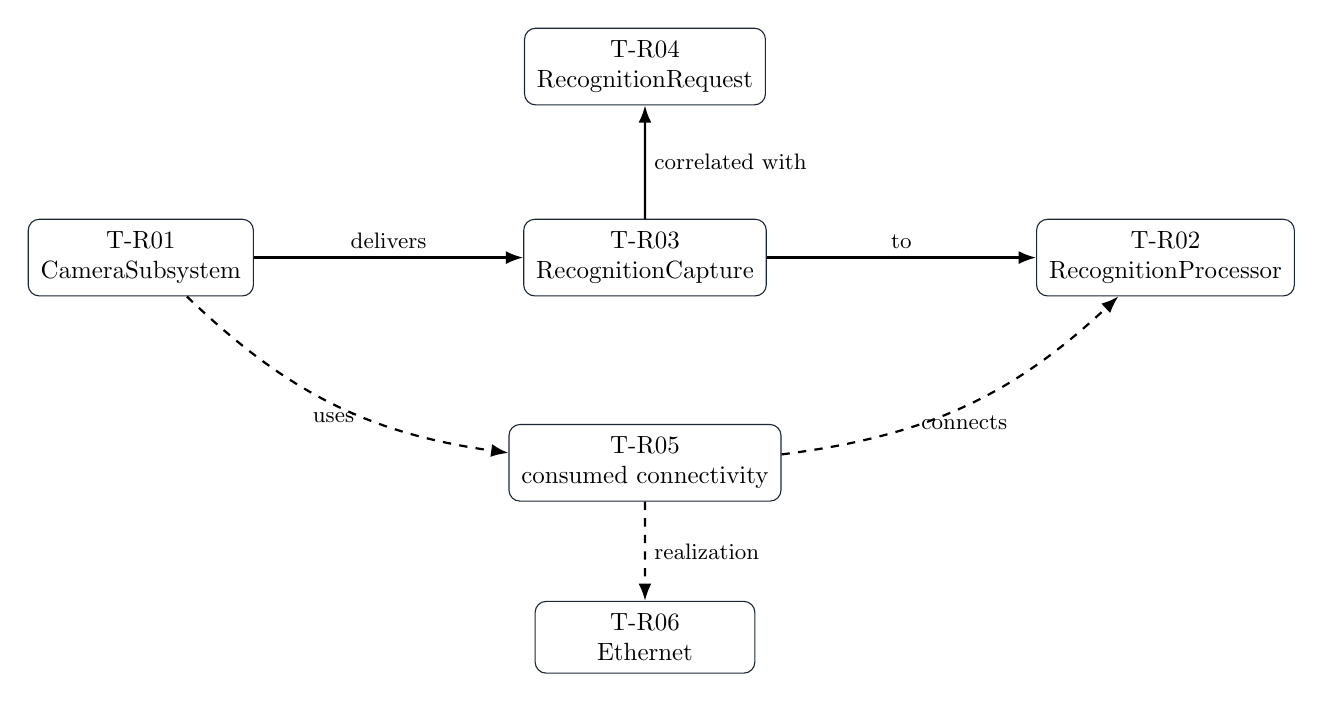
\begin{tikzpicture}[scale=0.90,transform shape,
 box/.style={draw=ddtadark,rounded corners,align=center,inner sep=5pt,minimum width=31mm},
 arr/.style={-{Latex[length=2.2mm]},thick},
 note/.style={font=\small,align=center},
 node distance=13mm and 18mm]
\node[box] (cam) {T-R01\\CameraSubsystem};
\node[box, right=38mm of cam] (cap) {T-R03\\RecognitionCapture};
\node[box, right=38mm of cap] (proc) {T-R02\\RecognitionProcessor};
\node[box, above=16mm of cap] (req) {T-R04\\RecognitionRequest};
\node[box, below=18mm of cap] (net) {T-R05\\consumed connectivity};
\node[box, below=14mm of net] (eth) {T-R06\\Ethernet};
\draw[arr] (cam)--node[above,note]{delivers}(cap);
\draw[arr] (cap)--node[above,note]{to}(proc);
\draw[arr] (cap)--node[right,note]{correlated with}(req);
\draw[arr,dashed] (cam) to[bend right=18] node[below,note]{uses}(net);
\draw[arr,dashed] (net) to[bend right=18] node[below,note]{connects}(proc);
\draw[arr,dashed] (net)--node[right,note]{realization}(eth);
\end{tikzpicture}
\end{center}

\begin{warningbox}{The diagram is not authority}
This rendering only visualizes the trial ledger. Source basis and analytical statements remain the semantic record.
\end{warningbox}

\section{Analytical-addition falsification probe}
A tool could invent \texttt{T-X01 RecognitionIngressEndpoint}. The selected source does not name or require an independently meaningful ingress endpoint.

\begin{lstlisting}
T-X01
origin      = A (candidate analytical addition)
accepted    = NO
reason      = baseline trial works without inventing it
\end{lstlisting}

The same applies to an invented first-class NetworkChannel. Transport semantics are real, but this trial does not force a channel entity with independent identity.

\section{Reuse test}
Two consumers reuse the same meaning without redefining it:

\begin{itemize}
\item \textbf{Consumer A - change-impact reasoning}: determines which statements survive Ethernet to Wi-Fi and which are revised.
\item \textbf{Consumer B - SpecializedRequirement applicability reasoning}: determines which delivery/payload/request meaning is constrained by SR-3.4-C/I/P and whether those obligations remain applicable after mutation.
\end{itemize}

\begin{resultbox}{T1 result}
A shared semantic contract is useful. T1 does not yet prove that DDTA must persist one long-lived materialized graph; a reproducibly rebuilt representation with stable identifiers remains a competing hypothesis.
\end{resultbox}

\section{Mutation M1 - Ethernet to Wi-Fi}
\small
\begin{longtable}{p{.25\textwidth}p{.17\textwidth}p{.38\textwidth}}
\toprule\textbf{Trial item} & \textbf{Result} & \textbf{Reason}\\\midrule\endhead
T-R01/T-R02 & RETAIN & same camera/processor separation\\
T-R03/T-R04 & RETAIN & same capture/request meaning\\
T-R05 & RETAIN & external ownership unchanged\\
T-R06 & REPLACE & Ethernet becomes Wi-Fi\\
T-S01..T-S05 & RETAIN & D-3.3, D-3.4 and FR-3.4 unchanged\\
T-S06 & REVISE & realization changed\\
T-S07..T-S09 & RETAIN after review & SRs retained in source regression\\
\bottomrule
\end{longtable}
\normalsize

M1 shows why stable analytical identity is useful while simultaneously showing that Ethernet/Wi-Fi need not be first-class BAEs.

\section{Mutation M3 - remote to local recognition}
\small
\begin{longtable}{p{.25\textwidth}p{.20\textwidth}p{.35\textwidth}}
\toprule\textbf{Trial item} & \textbf{Result} & \textbf{Reason}\\\midrule\endhead
T-R01 & RETAIN & camera remains relevant\\
T-R02 & REVIEW / MAY RETIRE OR MERGE & separate responsibility meaning changes\\
T-R03/T-R04 & REVIEW & local revised contract not inferred here\\
T-R05/T-R06 & REVIEW & may be irrelevant to capture transfer but not necessarily to all project use\\
T-S01 & RETIRE & old FR-3.4 retired/superseded\\
T-S02 & RETIRE WITH OLD FR & scoped to old delivery\\
T-S03 & REVISE/REPLACE & D-3.3 changed\\
T-S04 & RETIRE & old crossing disappears\\
T-S07..T-S09 & NOT APPLICABLE IN OLD FORM & source corpus says so\\
\bottomrule
\end{longtable}
\normalsize

M3 shows that stable identity requires semantic continuity, not string equality. The name \texttt{RecognitionProcessor} alone is insufficient to assert that the same analytical referent survives.

\section{Hypothesis results}
\begin{longtable}{p{.42\textwidth}p{.18\textwidth}p{.21\textwidth}}
\toprule\textbf{Hypothesis} & \textbf{T1 result} & \textbf{Effect}\\\midrule\endhead
Shared semantic contract is useful & SUPPORTED & keep in BA0\\
One persisted canonical graph is mandatory & NOT PROVEN / OPEN & weaken wording\\
Grounded / derived / addition distinction is useful & SUPPORTED WITH REFINEMENT & assertion-level origin pressure\\
Every useful responsibility needs first-class type & FALSIFIED & defer type decisions to BA1\\
Tool inference may become authority silently & REJECTED & T-X01 stays unaccepted\\
\bottomrule
\end{longtable}

\section{Revised BA0 candidate wording}
\begin{trialbox}{REVISED WORKING CANDIDATE / NOT CLOSED}
Base Analysis establishes an accepted, methodology-neutral analytical representation of the system knowledge needed by DDTA for a given governed baseline. The representation preserves shared analytical identity and the origin of analytical assertions, and can be reused or reproducibly rebuilt for multiple analysis consumers. It does not become a competing project source of truth, and no tool, view, method, or inferred structure may silently redefine its accepted meaning.
\end{trialbox}

The key change is:
\begin{lstlisting}
maintains one canonical persisted representation
    -> NOT REQUIRED BY T1

establishes shared accepted analytical identity/meaning
    -> SUPPORTED BY T1
\end{lstlisting}

\section{What remains untested}
\begin{itemize}
\item a real conflict between governed source claims;
\item a case where an analytical addition is necessary rather than merely convenient;
\item rename/refactoring identity rules;
\item persisted representation versus reproducible rebuild;
\item minimal BAE ontology, relation vocabulary, provenance implementation, views and threat overlays.
\end{itemize}

\section{Next microstep}
\textbf{BA0-T2 - conflict + necessary analytical-addition stress test.}

It will test one incompatible-source case, one genuinely necessary reviewed analytical addition, and a persisted-vs-rebuilt representation comparison. Only after T2 should BA0 be reconsidered for closure.

\enlargethispage{2\baselineskip}
\begin{resultbox}{State after BA0-T1}
\begin{lstlisting}
Chapters 2-4                      CLOSED / FINAL
Documentation layer               CLOSED
W0                                CLOSED
BA0-R systems-modeling prior art  CLOSED
BA0 working hypothesis R1         PRESERVED
BA0-T1 FR-3.4 application trial   COMPLETED / PROVISIONAL
BA0 responsibility/non-goals      REVISED WORKING CANDIDATE / NOT CLOSED
BA0-T2 conflict/addition trial    NEXT
BA1 minimal BAE ontology          NOT STARTED
BAE types accepted                 NONE
\end{lstlisting}
\end{resultbox}

\end{document}
